\chapter{Implementation}
\label{sec:implementation}

% Hier greift man einige wenige, interessante Gesichtspunkte der
% Implementierung heraus. Das Kapitel darf nicht mit Dokumentation oder
% gar Programmkommentaren verwechselt werden. Es kann vorkommen, daß
% sehr viele Gesichtspunkte aufgegriffen werden müssen, ist aber nicht
% sehr häufig. Zweck dieses Kapitels ist einerseits, glaubhaft zu
% machen, daß man es bei der Arbeit nicht mit einem "Papiertiger"
% sondern einem real existierenden System zu tun hat. Es ist sicherlich
% auch ein sehr wichtiger Text für jemanden, der die Arbeit später
% fortsetzt. Der dritte Gesichtspunkt dabei ist, einem Leser einen etwas
% tieferen Einblick in die Technik zu geben, mit der man sich hier
% beschäftigt. Schöne Bespiele sind "War Stories", also Dinge mit denen
% man besonders zu kämpfen hatte, oder eine konkrete, beispielhafte
% Verfeinerung einer der in Kapitel 3 vorgestellten Ideen. Auch hier
% gilt, mehr als 20 Seiten liest keiner, aber das ist hierbei nicht so
% schlimm, weil man die Lektüre ja einfach abbrechen kann, ohne den
% Faden zu verlieren. Vollständige Quellprogramme haben in einer Arbeit
% nichts zu suchen, auch nicht im Anhang, sondern gehören auf Rechner,
% auf denen man sie sich ansehen kann.

% Implementation motivation

While chapter \ref{sec:design} presented the design of the developed
system, this chapter will pick up some design details and focus on
their implementation.  It is not intended to provide a full
documentation of the developed source code, moreover it should be a
guide in understanding the system and also provide a basis for futher
developement. Therefore, documentation should be retrieved from the
source code or doxygen \cite{ref:doxygen} documentation.

The developement of the system started from the analysed requirements
of the PIConGPU source code (Section \ref{sec:picongpu}). Since,
PIConGPU is implemented in C / C++ and makes additional usage of the
Boost \cite{ref:boost} libraries, the same programming language was
also choosen for the implemenation of the system. Additional libraries were
selected with respect to the usage of similar design paradigms and an
easy integration into the C++ environment. Furthermore, should the
implementation make use of STL methods as often as possible to
gurantee easy integration into existing applications.  To make use of
a richer feature set of the C++ programming language, features of the
new C++11 standard were also included in the implementation
\cite{ref:c++11}.

The objective was to develope the designed system by a full functional prototype.
The prototype should be used to implement a simple example simulation
to proof functionality. The example should make use of all provided
communication features.

Particular C++ implementation details are highlighted by small source
code snippets, hence, a basic knowledge of the C++ programming
language and the dealing with templates is assumed.

%%%%%%%%%%%%%%%%%%%%%%%%%%%%%%%%%%%%%%%%%%%%%%%%%%%%%%%%%%%%%%%%%%%%%%%%%%%%%%%%
%                                                                              %
% CAL IMPLEMENTATION                                                           %
%                                                                              %
%%%%%%%%%%%%%%%%%%%%%%%%%%%%%%%%%%%%%%%%%%%%%%%%%%%%%%%%%%%%%%%%%%%%%%%%%%%%%%%%
\section{The CAL with Policy Based Design}

The communication abstraction layer was introduced in section
\ref{sec:cal} as a portable communication abstraction based on an
particular adapter. While the CAL defines the adapter interface, the adapter
implements communication operations based on an existing communication
library.  It was claimed, that the adapter should be exchangeable and
configurable at compile time. These requirements meet the properties of
a policy based design \cite{ref:policy_based_design}.

% Policy based design in general
Policy based design is a programming paradigm especially for the C++
programming language based on the concept of policy and host classes.
A policy is a class or class template interface, which consists of
inner type definitions, member functions and/or member variables. An
implementation of a policy is called policy class and is inherited by
or contained within a host class.  The advantage of policy based
design is that the functionality of the policy is bounded to its host
class at compile time, providing no runtime overhead.  The interface
of the policy is strictly defined by the host class. Ignoring this
interface leads to compile time errors. In summary, the host class
defines the interface of the policy, while the policy class implements
abitrary functionality against the policy interface. It is also called
the compile-time variant of the strategy pattern in
\cite{ref:policy_strategy}.

% Policy based design for CAL + adapter
Applying the policy based design on the design of the CAL
induces a allocation of roles, such that the CAL is the host class and
the adapter the communication policy. Figure \ref{fig:cal_uml} shows
the modeling of the CAL in an UML diagram. The CAL class is configurable by
an adapter class as template argument. At the same time it also inheritates
the properties of the adapter class in protected mode. Protected means
that only the CAL itself can access members of the adapter class.

\begin{figure}[H]
  \centering 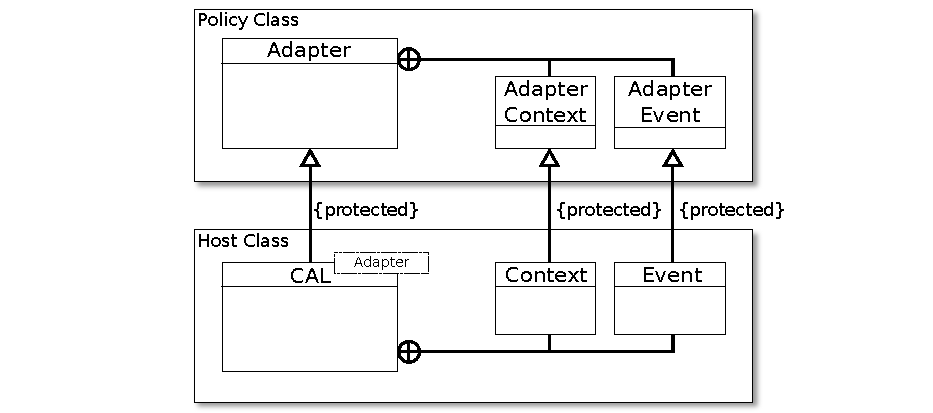
\includegraphics[width=\textwidth]{graphics/40_cal_uml}
  \caption{ }
  \label{fig:cal_uml}
\end{figure}

The CAL provides all communication methods discussed in section
\ref{sec:cal_comm} and context methods discussed in section
\ref{sec:cal_context}. The Adapter implements all methods
required by the communication policy defintion (Section \ref{sec:impl:policy_interface}).

In addition to communication and context related methods, the CAL
class provides class interface definitions of the context and the
event class. Both classes provide the interface claimed by the design
in sections \ref{sec:cal_context} and \ref{sec:cal_comm}. They
inheritate their functionality from equivalent classes in the adapter
class. Thus, an adapter has to implement an inner context and an inner
event class.  Figure \ref{fig:cal_uml} shows context and event of the
CAL class inheritating functionality of the equivalent classes in the
adapter class, also in protected mode. Section
\ref{sec:cal_mpi_adapter} will discuss the implementation of the
adapter specific context and event class implementation in detail.

% Policy interface
\subsubsection{Communication Policy interface}
\label{sec:impl:policy_interface}
\begin{itemize}
\item The policy interface was chosen to stay on a very low level
\item Because it should provide as much freedom to the adapter
  implementer as possible
\item Furthermore it was inspired by the sophisticated MPI language
  binding for C
\item Thus, it is more C then C++ like

\item A subset of adapter methods were chosen to
  illustrate the adapter interface

\item A full listing of all methods should be retrieved from
  the source code documentation

  \begin{itemize}
  \item Point-to-point operation\\
    \begin{lstlisting}[language=C++, breaklines=false, label={}]
Event asyncSendData(const T_Data* data,
                    const size_t count,
                    const VAddr destVAddr,
                    const T_Context context,
                    const MsgType msgType);
    \end{lstlisting}

  \item Collective operation\\
    \begin{lstlisting}[language=C++, breaklines=false, label={}]
void gather(const T_Data* sendData,
            const size_t sendCount,
            const T_Data* recvData,
            const size_t recvCount,
            const VAddr rootVAddr,
            const T_Context context);
    \end{lstlisting}
  \item Grouping operation\\
    \begin{lstlisting}[language=C++, breaklines=false, label={}]
      T_Context createContext(const std::vector<VAddr> vAddrs,
                              const T_Context oldContext);
    \end{lstlisting}
    
  \end{itemize}

\item Only a subset of operations known from MPI or other
  communication libraries have been implemented

\item Operations that were necessary during the implementation
  of the system and of example were implemented
  
\end{itemize}

% Addressing of peers
\subsubsection{Mapping to virtual addresses}
The the design chapter claimed the requirement for an unified address
space to uniquely address peers in a context of the CAL. The design decision
was to keep it as simple as possible. Thus, The address space of the
virtual addresses is in the range of natural numbers from 0 to the number
of peers minus one. An adapter has to make shure that its own address
space is mapped into the virtual address space.

% Description Communication operations
\subsubsection{Data Types}
All communication methods are able to transmit data objects from
abitrary data type defined by an template argument. The data object
has the interface requirement to provide both a pointer to the data
object memory and the amount of data objects. The method \cpp{data()}
should return the pointer and the method \cpp{size()} the number of
elements of with the template data type.Some containers of the
standard template library already provide those methods. Thus, data
can be easily encapsulated into \cpp{std::vector} or \cpp{std::array}
objects \cite{ref:vector, ref:array}. Listing \ref{lst:cal_async_send}
shows the implementation of the \cpp{asyncSend} method of the CAL.
\cpp{sendData} with data type \cpp{T_Data} provides both functions
claimed by the interface.

\begin{lstlisting}[language=C++, breaklines=false, label={lst:cal_async_send}]
template <typename T_Data>
Event asyncSend(const VAddr destVAddr, 
                const Tag tag, 
                const Context context, 
                const T_Data& sendData){

  return Event(
    CommunicationPolicy::asyncSendData(
      sendData.data(),
      sendData.size(), 
      destVAddr, 
      context, 
      tag
      
    )
      
  );

}
\end{lstlisting}

\subsubsection{Reduce operation}
A collective reduce operation is based on an binary operator. The C++
STL allready provides a handfull of binary functions in the functional
header like \cpp{std::plus}, \cpp{std::multiplies} or \cpp{std::minus}
\cite{ref:functional}. Functions that are not provided by the STL can
be easily created by an C++ struct or class overloading the bracket
operator. Listing \ref{lst:binary_function} shows a struct for
the maximum operator.

\begin{lstlisting}[language=C++, breaklines=false, label={lst:binary_function}]
template<typename T_Data>
struct maximum : public std::binary_function<T_Data, T_Data, T_Data> {

  // Bracket operator overloaded with binary operator for maximum
  const T_Data& operator()(const T_Data& x, const T_Data& y) const {
    return x < y? y : x;

  }

};
\end{lstlisting}

It can not be assumed that the general binary operator is supported by
every adapter specific reduce operation.  Thus, it may exist cases in
which the C++ binary operation has to be transformed to a adapter
specific one. In this cases, the tranformation logic needs to be
implemented inside the adapter class. Section \label{sec:bin_operator}
discusses the transformation for binary operators in the specific case
of a MPI adapter.

%%%%%%%%%%%%%%%%%%%%%%%%%%%%%%%%%%%%%%%%%%%%%%%%%%%%%%%%%%%%%%%%%%%%%%%%%%%%%%%%
%                                                                              %
% MPI ADAPTER                                                                  %
%                                                                              %
%%%%%%%%%%%%%%%%%%%%%%%%%%%%%%%%%%%%%%%%%%%%%%%%%%%%%%%%%%%%%%%%%%%%%%%%%%%%%%%%
\subsection{The MPI Adapter as Reference Implementation}
\label{sec:cal_mpi_adapter}

A reference adapter is described to give an insight into the
developement of an adapter and to give hints on parts of the adapter
implementation which should be considered carefully.  Further, the
description should give a guideline for the implementation of
additional adapter classes.

The reference adapter implementation is based on MPI as existing
communication layer.  MPI (Section \ref{sec:mpi}) was choosen,
because it already provides a lot of functionality required by the CAL
interface without any further effort. Additionally, it is available on wide range
of compute systems and can be used for free by open source
implementations. This section will make use of very MPI specifc 
vocabulary. It is assumed that the reader has a basic knowledge
on MPI terminology.

The instanctiation of a CAL object wit MPI adapter, also leads to an
initialization of the MPI adapter. The adapter creates the initial
global context by grouping all peers of MPI\_COMM\_WORLD.
Furthermore, a mapping from MPI ranks to virtual addresses for the
global context is created in the \cpp{vAddrMap}. Since, virtual
addresses are defined as natural number in the range from zero to the
numbers of peers minus one, the \cpp{AddrMap} is a one-to-one mapping
from virtual addresses to MPI ranks in a particular context.

\todo{implement Boost::mpi adapter}

The MPI C language binding is used inside the adapter to address the
message passing interface.  It provides the most general interface to
MPI and can by easily used in a C++ environment.  This interface is
very similar to the adapter interface. Thus, the implementation of the
adapter interface through MPI routines is not very
complex. Nevertheless, Listing \ref{lst:adapter_send} shows that the
\cpp{asyncSendData} method does not only forward to the MPI
communication operation \cpp{MPI_Issend}.  But also does a translation
from the virtual address \cpp{destVaddr} of a peer to the rank of an
MPI process through the vAddrMap at line~\ref{line:vAddrMap}, a
translation from the context to the MPI communicator at
line~\ref{line:contextMap} and the conversion of the data type
\cpp{T_Data} to an MPI data type at line~\ref{line:mpi_datatype}.  The
conversion of data types will be discussed in section
\ref{sec:data_type_conversion}.


\begin{lstlisting}[language=C++, breaklines=false, label={lst:adapter_send},escapechar=|]
template <typename T_Data, typename T_Context>      
Event asyncSendData(const T_data* const data, 
                    const size_t count, 
                    const Vaddr destVaddr, 
                    const T_Context context, 
                    const MsgType msg Type){    

  // Translation of vaddr to rank
  int destRank      = vAddrMap[context][destVaddr];|\label{line:vAddrMap}|

  // Translation of context to MPI Communicator
  MPI_Comm comm     = contextMap[context];|\label{line:contextMap}|

  // Conversion from T_Data to MPI data type
  MPI_Datatype type = ToMPIDatatype<T_Data>::type;|\label{line:mpi_datatype}|

  // MPI specific send operation                                                                            
  MPI_Request request; 
  MPI_Issend(const_cast<T_Data*>(data), 
             count, 
             type,
             destRank, 
             msgType,
             comm,
             &request);

  // Create and return event
  return Event(request);                                                                                                       

}  
\end{lstlisting}

The remaining adapter methods are implemented in a similar manner,
except for the reduce operation. Since the CAL interface accepts,
abitrary binary operators for the reduce collective, the MPI
adapter need to be able to handle these operators. Section
\ref{sec:bin_operator} covers the conversion from abitrary
binary operators to operators that can be used for MPI.

%%%%%%%%%%%%%%%%%%%%%%%%%%%%%%%%%%%%%%%%%%%%%%%%%%%%%%%%%%%%%%%%%%%%%%%%%%%%%%%%
%                                                                              %
% BINARY OPERATOR                                                              %
%                                                                              %
%%%%%%%%%%%%%%%%%%%%%%%%%%%%%%%%%%%%%%%%%%%%%%%%%%%%%%%%%%%%%%%%%%%%%%%%%%%%%%%%
\subsubsection{Binary Operator}
\label{sec:bin_operator}

MPI has built-in support for binary operations by two approaches. The
simplest approach, is the direct usage of predefined binary MPI
operators\cite{ref:mpi_bin_op}. But, since the system user should not
use specific MPI operators, the CAL could wrap all available MPI
operators in a struct of static const expressions (Listing
\ref{lst:mpi_bin}).  The CAL could forward the struct to the user of
the system and the user could select from these binary operations
depending on the reduction operation. Reduction by accumulation would
use the \cpp{BinaryOperations::SUM} operator.


\begin{lstlisting}[language=C++, caption={A small collection of binary operators by transformed MPI operations to static constexpression }, label=lst:mpi_bin]
struct BinaryOperations { 
  static constexpr BinaryOperation MAX = MPI_MAX; 
  static constexpr BinaryOperation MIN = MPI_MIN; 
  static constexpr BinaryOperation SUM = MPI_SUM; 
  static constexpr BinaryOperation PROD = MPI_PROD; 
  ...

};
\end{lstlisting}


The downside of the this approach is that only the 12 predefined
operators of MPI can be used, restricting the application on this
limited set of operators. Therfore, MPI gives the possibility to
create abitrary binary operators with the \cpp{MPI\_Op\_create}
function.  The source code for transforming abitrary binary operators
to binary MPI operators was taken over from the boost::mpi project
\cite{ref:boost_mpi} and adapted for the needs of the MPI adapter.
Listing \ref{lst:mpi_bin2} shows the transformation of a binary C++
\cpp{operator} from type \cpp{T\_BinaryOperation} with data type
\cpp{T\_Data} to \cpp{MPIoperator} from type {MPI\_Op}.  After the
transformation, the MPI operator can be retrieved by
\cpp{MPIOperator.getOperator} and then used by all MPI routines that
are using binary operators.

\begin{lstlisting}[language=C++, caption={ }, label=lst:mpi_bin2]
// Transformation of binary operator
toMPIOperator<T_Data, T_BinaryOperator> MPIOperator(operator);

// Retrieve binary MPI operator
MPIOperator.getOperator()
\end{lstlisting}


The second approach is essentially more flexible then the first
one. Thus, it was chooses to implement binary operations for the
MPI adapter.

%%%%%%%%%%%%%%%%%%%%%%%%%%%%%%%%%%%%%%%%%%%%%%%%%%%%%%%%%%%%%%%%%%%%%%%%%%%%%%%%
%                                                                              %
% DATA TYPE CONVERSION                                                         %
%                                                                              %
%%%%%%%%%%%%%%%%%%%%%%%%%%%%%%%%%%%%%%%%%%%%%%%%%%%%%%%%%%%%%%%%%%%%%%%%%%%%%%%%
\subsubsection{Data Type Conversion}
\label{sec:data_type_conversion}
MPI predefines on one hand its primitive data types, but on the other
hand also provides the possibility to define own data structures based
upon sequences of the MPI primitive data types. Such user defined data
structures are called derived data types. Usually, Primitive data
types are contiguous. But, derived data types allow you to specify
non-contiguous data in a confortable manner and to treat it as though
it was contiguous.  Thefore, more complex data types (e.g structs or
classes) can be transformed into derived data types. The exchange
of complex data types was not necessary in the developement of the
system based on examples of section \ref{sec:gol_imp}. Thus, the
implementation was focused on the transformation of primitive data
types.  But nevertheless, a transformation is available in the
boost::mpi \cite{ref:boost_mpi} implementation. Thus switching to
boost::mpi or adopting their source code would solve this problem
without any further effort.

The primitive C++ data types can be mapped directly to primitive MPI
data types. By the fact, that MPI data types are defined by C macros,
a C++ data type need to be converted to an integer number. The
conversion is implemented by the concept of type traits
\cite{ref:type_trait}.  Type traits are classes that obtain
characteristics of types in the form of compile-time constant values.

The function of the type trait is the transformation of primitive C++
data types to predefined MPI data types.  First, a template struct
defines the default behaviour of the type trait (Listing
\ref{lst:mpi_trait1}). The struct defines a static const expression
\cpp{type}, which is set to a fixed MPI data type. The template
argument \cpp{T_Data} is the primitive C++ data type that should be
transformed. The default struct will transform abitrary data types
\cpp{T_Data} to the \cpp{MPI\_CHAR} data type. The MPI data type of
\cpp{T_Data} can be retrieved by \cpp{ToMPIDatatype<T_Data>:type}.


\begin{lstlisting}[language=C++, label=lst:mpi_trait1]
  template<typename T_Data> 
  struct ToMpiDatatype { 

    static constexpr MPI_Datatype type = MPI_CHAR; 

  };
\end{lstlisting}


The template in listing \ref{lst:mpi_trait2} is a explicit
specialization of the default template in listing
\ref{lst:mpi_trait1}. In this case, a specialization for the C++ data
type \cpp{int}, which will be transformed to the \cpp{MPI\_INT} data type.  Thus,
each transformation of a primitive C++ data type need to be defined
by its own specialisation template, assumed that a corresponding
MPI data type exists.

\begin{lstlisting}[language=C++, label=lst:mpi_trait2]
  template<>
  struct ToMPIDatatypes<int> { 

    static constexpr MPI_Datatype type = MPI_INT; 

  };
\end{lstlisting}

The communication operations within the adapter uses the type trait to
tranform the data types of the input and output data, by querying the
type trait. Listing \ref{lst:mpi_trait3} gives an example for the conversion 
of the C++ data type \cpp{int}.

\begin{lstlisting}[language=C++, label=lst:mpi_trait3]
  MPI_Datatype type = ToMPIDataType<int>::type;
\end{lstlisting}

%%%%%%%%%%%%%%%%%%%%%%%%%%%%%%%%%%%%%%%%%%%%%%%%%%%%%%%%%%%%%%%%%%%%%%%%%%%%%%%%
%                                                                              %
% CONTEXT EVENT MPI ADAPTER                                                    %
%                                                                              %
%%%%%%%%%%%%%%%%%%%%%%%%%%%%%%%%%%%%%%%%%%%%%%%%%%%%%%%%%%%%%%%%%%%%%%%%%%%%%%%%
\subsubsection{Context and Event in MPI Adapter}
The MPI adapter specific event makes use of MPI non-blocking
communication features. In the MPI world, a non-blocking function
returns a request object, which is the handle to verify the state of
the function. The wait method is implemented by a \cpp{MPI\_Wait} on
the request:

\begin{lstlisting}[language=C++, label=lst:mpi_event_wait]
void wait(){
  MPI_Status status;
  MPI_Wait(&request, &status);

}
\end{lstlisting}

The ready methods checks with \cpp{MPI\_Test} whether the function has
already finished:

\begin{lstlisting}[language=C++, label=lst:mpi_event_ready]
bool ready(){
  int flag = 0;
  MPI_Status status;
  MPI_Test(&request, &flag, &status);
  return bool(flag);

}
\end{lstlisting}

%%%%%%%%%%%%%%%%%%%%%%%%%%%%%%%%%%%%%%%%%%%%%%%%%%%%%%%%%%%%%%%%%%%%%%%%%%%%%%%%
%                                                                              %
% GRAPH IMPLEMENTATION                                                         %
%                                                                              %
%%%%%%%%%%%%%%%%%%%%%%%%%%%%%%%%%%%%%%%%%%%%%%%%%%%%%%%%%%%%%%%%%%%%%%%%%%%%%%%%
\section{Graph Based on the Boost Graph Library}

Section \ref{sec:graph} introduced a graph interface.  This graph
interface is implemented on basis of an existing graph library as
backend. It can be choosen from a range of different graph libraries
like \cite{ref:lemon, ref:boost_bgl, ref:igraph, ref:ogdf}.
Since, the boost project is closely related to the C++ standard
template library, the Boost Graph Library \cite{ref:boost_bgl}, short
BGL, was selected as graph backend.

While the BGL provides a powerful interface and a wide range of graph
algorithms, just a small subset of this functionality is really
necessary for the purposes of this work. Thus, the BGL is wrapped
inside a graph class providing common graph funcionality.  The
graph class provides all claimed methods discussed in design section
\ref{sec:graph}, but the methods are handled by the Boost Graph Library.


%%%%%%%%%%%%%%%%%%%%%%%%%%%%%%%%%%%%%%%%%%%%%%%%%%%%%%%%%%%%%%%%%%%%%%%%%%%%%%%%
%                                                                              %
% PROPERTIES                                                                   %
%                                                                              %
%%%%%%%%%%%%%%%%%%%%%%%%%%%%%%%%%%%%%%%%%%%%%%%%%%%%%%%%%%%%%%%%%%%%%%%%%%%%%%%%
\subsection{Vertices Annotated by Properties}

A graph can be anotated by properties that are used to describe
vertices and edges with simulation specific information, like
discussed in section \ref{sec:graph}. Vertices and edges are
configured by properties at compile time through template
parameter. In the wrapper graph implementation, vertices and edges are
represented by the property itself. Whereby, The BGL refers to
vertices and edges by indices of integer numbers, whereby properties
of this vertices can be queried from so called property maps.

The implementation of a property is a struct or a class with abitrary content. It need
to provide an id member variable to create an internal connection of
the property to the vertex index of the BGL.  The most simple property
is a struct only containing the id, like presented in listing
\ref{lst:property}. This property is predefined in the graph
header. It is used as default when the graph is configured without any
declaration of a property.

\begin{lstlisting}[language=C++, label=lst:property]
struct SimpleProperty {

    SimpleProperty() : id(0) {

    }
    
    SimpleProperty(ID id) : id(id) {

    }

    // Vertex id refers to BGL vertex index
    unsigned id;
};
\end{lstlisting}

Requesting the vertices of the graph, returns a vector with all
vertices of the graph. But, that vector is actually a list of vertex
properties in the context of the BGL, whereby every property is
connected by its id to the graph. This connection is transparent for
the the system user, hence, the user do not have to care about it.

%%%%%%%%%%%%%%%%%%%%%%%%%%%%%%%%%%%%%%%%%%%%%%%%%%%%%%%%%%%%%%%%%%%%%%%%%%%%%%%%
%                                                                              %
% CREATION OF A GRAPH                                                          %
%                                                                              %
%%%%%%%%%%%%%%%%%%%%%%%%%%%%%%%%%%%%%%%%%%%%%%%%%%%%%%%%%%%%%%%%%%%%%%%%%%%%%%%%
\subsection{Creation of a Graph}
A graph is created by a list of edge descriptors and a list of
corresponding vertices. An edge descriptor is the tuple of source
vertex, destination vertex and the connecting edge. The list of edge
descriptors can also be generated by a graph generator. A set
generators for commonly used graph topologies is already implemented
(Figure \ref{fig:topologies}).  The set of generators covers fully
connected topologie, star topology, n-dimensional hypercube topologie
and n-dimensional grid topology.  The generators are parametrizable by
number of vertices and/or dimension.  The functions that generate a
topology have the advantage that they can be reused in different
applications with same communication topology.

\begin{figure}[H]
  \centering
  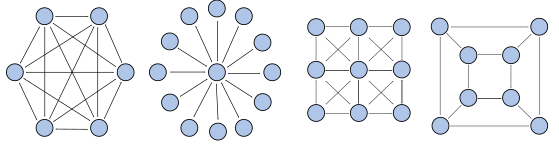
\includegraphics[width=\textwidth]{graphics/40_topologies}
  \caption{Set of already implemented graph generators. Nevertheless,
  abitrary graphs can be generated by user defined generator functions.}
  \label{fig:topologies}
\end{figure}

%%%%%%%%%%%%%%%%%%%%%%%%%%%%%%%%%%%%%%%%%%%%%%%%%%%%%%%%%%%%%%%%%%%%%%%%%%%%%%%%
%                                                                              %
% CREATION OF SUBGRAPHS                                                        %
%                                                                              %
%%%%%%%%%%%%%%%%%%%%%%%%%%%%%%%%%%%%%%%%%%%%%%%%%%%%%%%%%%%%%%%%%%%%%%%%%%%%%%%%
\subsection{Creation of a Subgraph}
The creation of a subgraph plays an important role for collective
operations on a subset of graph vertices. A subgraph can be created
from its supergraph by a subset of its vertices.  The creation of
subgraphs is meant to be used as an equivalent to the creation of
contexts in the CAL. Collective operations on this subgraph only
consider vertices within this subgraph. The BGL has already builtin
support for subgraphs.

A created subgraph is linked to its supergraph, whereby each graph
holds a list of its subgraphs. The connection of super and subgraph is
important for the context creation in collective operations in section
\ref{sec:gvon_impl}, because the announcement of a subgraph considers
first of all the context of the supergraph. Figure
\ref{fig:subgraph_creation} shows the creation of a two-dimensional
hypercube subgraph from a three dimensional hypercube supergraph.

\begin{figure}[H]
  \centering
  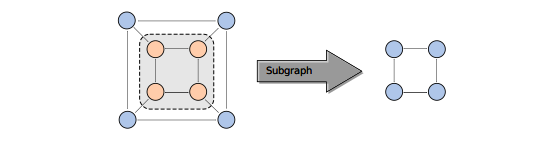
\includegraphics[width=\textwidth]{graphics/40_subgraph_creation}
  \caption{Inner vertices of a three-dimensional hypercube graph are 
  transformed to a two-dimensional hypercube subgraph. Both graphs
  stay connected by the BGL.}
  \label{fig:subgraph_creation}
\end{figure}

%%%%%%%%%%%%%%%%%%%%%%%%%%%%%%%%%%%%%%%%%%%%%%%%%%%%%%%%%%%%%%%%%%%%%%%%%%%%%%%%
%                                                                              %
% GRAPH BASED VIRTUAL OVERLAY NETWORK                                          %
%                                                                              %
%%%%%%%%%%%%%%%%%%%%%%%%%%%%%%%%%%%%%%%%%%%%%%%%%%%%%%%%%%%%%%%%%%%%%%%%%%%%%%%%
\section{Graph-Based Virtual Overlay Network}
\label{sec:gvon_impl}

The graph-based virtual overlay network was claimed as a combination
of graph and CAL. The combination is the connection of graph and CAL
by several mapping. These mappings are core components of the GVON and
are filled by the announcement process, which implementation is
discussed in section \ref{sec:announcement_impl}. In the following
each map is described:

\paragraph*{}
The \cpp{vertexMap} is a mapping from a vertex of a graph to the virtual
address of its host.  This map is used for all methods
that need to resolv the host of a vertex.
\begin{lstlisting}[language=C++, label=lst:mapping1]
std::map<Graph, std::map<Vertex, VAddr> > vertexMap;
\end{lstlisting}

\paragraph*{}
The \cpp{graphMap} is a mapping from a graph to its related context
created in the announcement process. This map is important since only
the hosts of a graph are related to communication processes of the
graph. Thus, a context covering only hosts of the graph need to be
resolved.
\begin{lstlisting}[language=C++, label=lst:mapping2]
std::map<Graph, Context> graphMap;
\end{lstlisting}

\paragraph*{}
The \cpp{peerMap} is kind of a reverse mapping of the \cpp{vertexMap}.
This map is a mapping from peers to its hosted vertices for a
particular graph.
\begin{lstlisting}[language=C++, label=lst:mapping3]
std::map<Graph, std::map<VAddr, std::vector<Vertex>> > peerMap 
\end{lstlisting}

\paragraph*{}
Listing \ref{lst:comm_gvon} shows the \cpp{asyncSend} method of the
GVON, the vertex is translated to its hosts virtual address in line
\ref{line:gvon_async_send1}, the graph is translated to its context
in line \ref{line:gvon_async_send2}.
\begin{lstlisting}[language=C++, label=lst:comm_gvon,escapechar=|]
template <typename T_Data>
Event asyncSend(Graph& grpaph, 
                const Vertex destVertex, 
                const Edge edge, 
                const T_Data& data){ 

  // Retrieve host virtual address of destVertex in graph
  VAddr destVAddr = vertexMap[graph][destVertex];|\label{line:gvon_async_send1}|

  // Retrieve context of the graph
  Context context = contextMap[graph];|\label{line:gvon_async_send2}|

  // Use CAL to send data
  return cal.asyncSend(destVAddr, edge.id, context, data);

}
\end{lstlisting}

Collective operations make also use of the GVON maps, but its
impelmentation is far more complex and therefore discussed in detail
in section \ref{sec:gvon_collective}.


%%%%%%%%%%%%%%%%%%%%%%%%%%%%%%%%%%%%%%%%%%%%%%%%%%%%%%%%%%%%%%%%%%%%%%%%%%%%%%%%
%                                                                              %
% ANNOUNCEMENT PROCESS                                                         % 
%                                                                              %
%%%%%%%%%%%%%%%%%%%%%%%%%%%%%%%%%%%%%%%%%%%%%%%%%%%%%%%%%%%%%%%%%%%%%%%%%%%%%%%%
\subsection{Announcement Process of Graphs}
\label{sec:announcement_impl}

The GVON interface provide an announcement method for the construction
of the mapping from vertices to peers of a context in the vertexMap
and the mapping from graphs to new created contexts in the graphMap.
The method takes a the pair of a graph and a vector of vertices as
input arguments. This has the meaning that the peer, calling the
announce method, wants host these vertices of the graph.  It is a
collective operation of all the peers that want to take part on the
communication of a particular graph.

These peers create first and foremost an exclusive context for
themselves, which only contains hosts of the graph that will be
announced.  Therfore the most general context of the hosts, possibly
including more peers, has to be determined.  The overall most general
context is the global context of all peers in the network, but in some
cases exists also a context with less peers.  This is either the
context of the graph or the context of the supergraph, if these graphs
were already announced.

Afterwards a new context is created from the present most general one
by gathering the number of hosted vertices from each peer and every
peer that hosts at least one vertex will belong to the new context.
Finally, The graph is mapped to the new context in the graph map and
will be used on further communication operations including this graph.


%%%%%%%%%%%%%%%%%%%%%%%%%%%%%%%%%%%%%%%%%%%%%%%%%%%%%%%%%%%%%%%%%%%%%%%%%%%%%%%%
%                                                                              %
% COLLECVITE OPERATIONS LOCALLY                                                %
%                                                                              %
%%%%%%%%%%%%%%%%%%%%%%%%%%%%%%%%%%%%%%%%%%%%%%%%%%%%%%%%%%%%%%%%%%%%%%%%%%%%%%%%
\subsection{Collective Operations on Graphs}
\label{sec:gvon_collective}

Because peers host potentially more than one vertex, collective
operation have to be performed locally first. This means, that data of
each hosted vertex has to be collected locally.  The implementation is
a bit tricky because the data has an abitrary data type. Thus, the
data from hosted vertices is collected in a templated collector until
all hosted vertices of this host have terminated their collective
operation.

\paragraph*{}
The collector is a templated static object from type \cpp{Collective}:
\begin{lstlisting}[language=C++, label=lst:static_collective]
// Type dependent instanciation of Collective class
static Collective<T_Data> collector;
\end{lstlisting}

\paragraph*{}
A \cpp{Collective} is templated struct thats can store data of type
\cpp{T_Data} for a root vertex (Listing \ref{lst:collective}). The data is
pushed to the data vector and the memory address of the receive vector
of the root vertex is stored in \cpp{rootPtr}.
\begin{lstlisting}[language=C++, label=lst:collective]
template <typename T_Data> struct Collective { 

  // Vector for collected data
  std::vector<T_Data> data; 

  // Pointer to vector of root vertex
  std::vector<T_Data>* rootPtr; 

};
\end{lstlisting}

\paragraph*{}
Each call of a collective operation is then collecting the data of the
calling vertex by the collector (Listing \ref{lst:collecting}).  In
case the the root vertex is calling the operation, the receive pointer
of the root vertex is stored.
\begin{lstlisting}[language=C++, label=lst:collecting]
// Collection of vertex data
collector.data.push_back(vertexData);
\end{lstlisting}

A peer could try to mix the execution of collective operations of
several graphs. But, it is only one collective per pair of a graph and
a vertex allowed concurrently. To ensure that, the amount of already
executed collective operations per vertex on a graph is counted.  Is
this count at the beginning of a collective greater than zero, then
the collective execution is aborted by an exception.

When the last vertex terminates its collective operation, the
operation is executed locally and then forwarded to the CAL
interface. The CAL then executes the collective operation among all
other hosts of the graph and returns the result. For collectives like
gather, the resulting data is reorder such that the gvon returns the
data in vertex id order. Finally, the result is written to the receive
pointer of the root vertex stored in the collector.


%%%%%%%%%%%%%%%%%%%%%%%%%%%%%%%%%%%%%%%%%%%%%%%%%%%%%%%%%%%%%%%%%%%%%%%%%%%%%%%%
%                                                                              %
% GAME OF LIFE IMPLEMENTATION                                                  %
%                                                                              %
%%%%%%%%%%%%%%%%%%%%%%%%%%%%%%%%%%%%%%%%%%%%%%%%%%%%%%%%%%%%%%%%%%%%%%%%%%%%%%%%

\section{Implementing a Game of Life}
The Game of Life simulation was implemented to show the developed
system in a real world scenario. The set of rules based on \cite{ref:gol_rules}
is listed in the following:

\begin{enumerate}
\item Any live cell with fewer than two live neighbours dies, as if caused by under-population.
\item Any live cell with two or three live neighbours lives on to the next generation.
\item Any live cell with more than three live neighbours dies, as if by overcrowding.
\item Any dead cell with exactly three live neighbours becomes a live cell, as if by reproduction.
\end{enumerate}

%%%%%%%%%%%%%%%%%%%%%%%%%%%%%%%%%%%%%%%%%%%%%%%%%%%%%%%%%%%%%%%%%%%%%%%%%%%%%%%%
%                                                                              %
% CONFIGURATION AND INITIALIZATION OF GOL                                      %
%                                                                              %
%%%%%%%%%%%%%%%%%%%%%%%%%%%%%%%%%%%%%%%%%%%%%%%%%%%%%%%%%%%%%%%%%%%%%%%%%%%%%%%%
\subsection{Configuration and Initialization of Game of Life}
The following source code describes necessary steps to configure and
initialize the system before starting the communication of GoL. The
source code is specific for the presented MPI adapter, GoL graph and
cell property. It should demonstrate the general programm flow and be
the foundation for usage in other simulation applications.

\begin{enumerate}

\item \textbf{Configuration}
\begin{enumerate}

\item Configure the CAL
  
  The Target system for the example is a compute cluster providing MPI
  as communication library. Thus, the CAL is configured with the
  reference MPI adapter described in section
  \ref{sec:cal_mpi_adapter}. It provides type definitions for the
  virtual address, event and context that are necessary for
  later usage:

  \begin{lstlisting}[language=C++, label=lst:conf_cal, caption={\ }]
// Configure CAL
typedef CommunicationPolicy::MPI                  Mpi;
typedef CommunicationAbstractionLayer<Mpi>        MpiCAL;
typedef typename MpiCAL::VAddr                    VAddr;
typedef typename MpiCAL::Event                    Event;
  \end{lstlisting}

\item Configure graph

  The graph is configured with properties for vertices \cpp{Cell}
  (Listing \ref{lst:gol_cell}) and edges \cpp{SimpleProperty}. It
  provides type definitions for vertex, edge and edge descriptor:

  \begin{lstlisting}[language=C++, label=lst:conf_graph, caption={\ }]
// Configure graph
typedef Graph<Cell, SimpleProperty>               LifeGraph;
typedef typename LifeGraph::Vertex                Vertex;
typedef typename LifeGraph::Edge                  Edge;
typedef typename LifeGraph::EdgeDescriptor        EDesc;
  \end{lstlisting}

  A \cpp{Cell} does contain the state information of the cell, theand
  inherits from \cpp{SimpleProperty} the vertex id. 31.25
  percent of all cells are initialized with state alive set to true.

\begin{lstlisting}[language=C++, label=lst:gol_cell, caption={\ }]
struct Cell : public SimpleProperty { 

 Cell() : SimpleProperty(0), isAlive(false){ 
          
 }
        
 // Initialization of the cell
 Cell(ID id) : SimpleProperty(id), isAlive(false){ 
   unsigned random = rand() % 10000;
   if(random < 3125){ 
     isAlive = true;
     
   }
   
 }

 // State of the cell
 bool isAlive;
 
};
\end{lstlisting}

\item Configure GVON

  The graph-based virtual overlay network uses the previously configured
  CAL and graph for its configuration:

  \begin{lstlisting}[language=C++, label=lst:conf_gvon, caption={\ }]
// Configure GVON
typedef VirtualOverlayNetwork<LifeGraph, MpiCAL>  GVON;
  \end{lstlisting}

\end{enumerate}

\item \textbf{Initialization}
  \begin{enumerate}
  
  \item Create graph object

    The graph is generated by the predefined graph generator for grids
    (Listing \ref{lst:gol_generator_graph}). The generator was
    configured to create a two dimensional grid , while diagonal
    arranged cells are connected (similar to Figure \ref{fig:gol_modeling}).

  \begin{lstlisting}[language=C++, label=lst:gol_generator_graph, caption={\ }]
// STL namespace
using namespace std;

// Generate GoL graph
vector<Vertex> vertices;
vector<EDesc> edges = Topo::gridDiagonal<LifeGraph>(n, vertices);
LifeGraph graph (edges, vertices); 
  \end{lstlisting}

\item Create CAL and GVON objects

  \begin{lstlisting}[language=C++, label=lst:, caption={\ }]
// Instanciate CAL and GVON
MpiCAL cal;
GVON gvon(cal);
  \end{lstlisting}

\item Distribute vertices of the graph

  The graph vertices are distributed by the round-robin method for
  testing, which is by far no optimal vertex distribution method, but
  this is not the focus of this work (Listing \ref{lst:gol_distribution}).  

  \begin{lstlisting}[language=C++, label=lst:gol_distribution, caption={\ }]
// Distribution of graph by round-robin
Context context = cal.getGlobalContext();
vector<Vertex> hostedVertices = Dist::roundrobin(context, graph);
  \end{lstlisting}

  Other abitrary distribution methods are also possible. Figure
  \ref{fig:gol_mapping} shows two different vertex distributions
  methods.  In the first distribution, hosted vertices are connected
  within the same host, since this reduces communication operations
  with other peers.  In the second distribution every vertex ist
  hosted by exactly one peer, representing a case where the graph
  represents exactly the communicating processes.

  \begin{figure}[H]
    \centering
    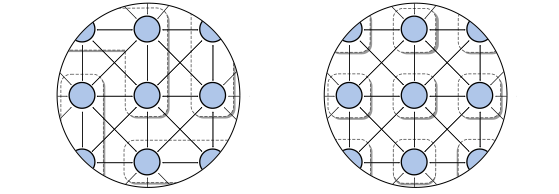
\includegraphics[width=\textwidth]{graphics/40_gol_mapping}
    \caption{Cut out of a GoL world. Possible distribution of modelled
      GoL graph. On the left side a peer host a connected set of
      vertices. While, on the right side, every peer hosts exactly one
      vertex.}
    \label{fig:gol_mapping}
  \end{figure}

  The distribution scales from one host that hosts all vertices to the
  number of hosts where every host get exactly one
  vertex. Distributing the graph to more peers than available vertices
  is an interessting case for fault tolerance and load balancing. Thus
  additional peers could be used as backup peers, but this is left
  open for future work.  After distribution vertices, every peer
  announces its vertices to the GVON (Listing \ref{lst:gol_announce}).

\item Announcement of hosted vertices
  \begin{lstlisting}[language=C++, label=lst:gol_announce, caption={\ }]
// Announcement of hosted vertices
gvon.announce(graph, hostedVertices);
  \end{lstlisting}
  \end{enumerate}
\end{enumerate}

%%%%%%%%%%%%%%%%%%%%%%%%%%%%%%%%%%%%%%%%%%%%%%%%%%%%%%%%%%%%%%%%%%%%%%%%%%%%%%%%
%                                                                              %
% COMMUNICATION OF GAME OF LIFE                                                %
%                                                                              %
%%%%%%%%%%%%%%%%%%%%%%%%%%%%%%%%%%%%%%%%%%%%%%%%%%%%%%%%%%%%%%%%%%%%%%%%%%%%%%%%
\subsection{Communication of Game of Life}
\label{sec:gol_imp}
Since the rules only require next neighbor communication, the GoL
domain is modeled as a two-dimensional grid with diagonal connections
like the unbundled version in section \ref{sec:gol}. Thus, a GoL cell
is represented by a vertex and neighboring cells are connected by
edges. A cell has to communicate with its neighboring cells and
retrieve their state to calculate its own state for the next time
step.

In the following the implementation of a single evolution step of GoL
is described. The Communication between vertices of the GoL graph
is handled by the GVON. A host has a list of its hosted vertices it is
responsible for. Thus, a host has to manage the communication of its
hosted vertices. In the case of GoL, a host has to exchange the state
of its hosted cells with neihboring cells.

\paragraph*{}
First, each host sends the state of its hosted cells to neihboring
cells (Listing \ref{lst:gol_send}). Therefore, the host retrieves the
target cells of outgoing edges for a hosted cell from the graph. After
that, the state of the hosted cell is transmitted to the target cells
sequentially in non blocking mode (Figure
\ref{fig:gol_communication}). Events of the send operation are
collected and checked later for termination.

\begin{lstlisting}[language=C++, label=lst:gol_send, caption={\ }]
// Send state to neighbor cells
for(Vertex v : hostedVertices){
  for(std::pair<Vertex, Edge> edge : graph.getOutEdges(v)){
    events.push_back(
      gvon.asyncSend(graph, edge.first, edge.second, v.isAlive)
    );

  }

}
\end{lstlisting}

\paragraph*{}
Second, each peer has to receive state information from neighboring
cells for each of its hosted cells (Listing
\ref{lst:gol_recv}). Therefore, the peer queries the source cell of
incoming edges for its hosted cells from the graph. Further, it
receives the state information from this neighboring source cells.
The receive operation is used in blocking mode, thus, all peers are
synchronized afterwards.

\begin{lstlisting}[language=C++, label=lst:gol_recv, caption={\ }]
// Recv state from neighbor cells
for(Vertex &v : hostedVertices){
  for(std::pair<Vertex, Edge> edge : graph.getInEdges(v)){
    gvon.recv(graph, edge.first, edge.second, edge.first.isAlive);
    if(edge.first.isAlive[0]) { 
      v.aliveNeighbors++;

  }

}
\end{lstlisting}

Figure \ref{fig:gol_communication} shows the sending process of a host
for each of its hosted vertices.

\begin{figure}[H]
  \centering
  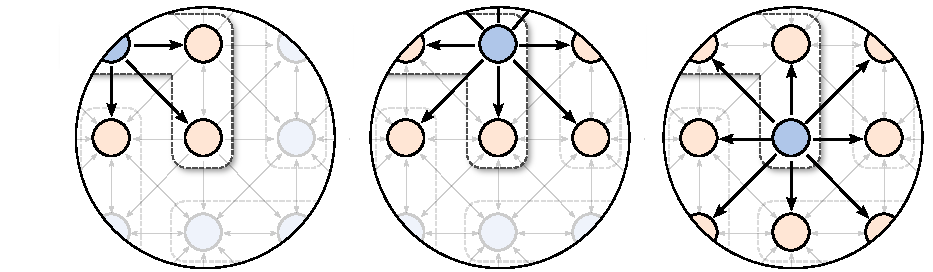
\includegraphics[width=\textwidth]{graphics/40_gol_communication}
  \caption{Cut out of a GoL world. A peer sends status information of
    hosted cells to neighboring cells. The communication operations
    are executed sequentially, but non blocking. Receive operations
    behave analog, but in blocking mode.}
  \label{fig:gol_communication}
\end{figure}

Once all send and receive operations have finished, the peer updates
the state of its hosted cells by the state of their neihboring cells
in dependence of the introduced rules. Finally the state information
of all cells is gathered by a abitrary cell which prints it to the
console for visualization and all hosts synchonize their program flow
(Listing \ref{lst:gol_gather}). The next evolution steps will repeat the
previous steps until the application is aborted or a fixed number of
evolutions steps is reached.

\begin{lstlisting}[language=C++, label=lst:gol_gather, caption={\ } ]
// Gather state by vertex with id = 0
for(Vertex v: hostedVertices){
  gvon.gather(graph.getVertices().at(0), v, graph, v.isAlive[0], golDomain);

}
\end{lstlisting}


%%%%%%%%%%%%%%%%%%%%%%%%%%%%%%%%%%%%%%%%%%%%%%%%%%%%%%%%%%%%%%%%%%%%%%%%%%%%%%%%
%                                                                              %
% Implementation N-BODY                                                        %
%                                                                              %
%%%%%%%%%%%%%%%%%%%%%%%%%%%%%%%%%%%%%%%%%%%%%%%%%%%%%%%%%%%%%%%%%%%%%%%%%%%%%%%%
\section{Implementing a N-Body Simulation}
\begin{itemize}
\item The implementation of the n body simulation, discussed in
  section \ref{sec:design:nbody}, does not differ very much from the
  GoL implementation in the fashion it uses the developed system.

\item The implementation is separated in three phases: Configuration, initialization
  and communication.

  \begin{enumerate}
  \item \textbf{Configuration}\\
    The Graph is annotated by the property \cpp{Particle}, containing
    Particle information mass, velocity and location.

  \item \textbf{Initialization}\\
    Since, the chosen N-body algorithm is based on an all to all communication
    schema, the communication dependencies are described by an fully connected
    graph. The vertices are distributed by round-robin onto the available
    peers and then announced.

  \item \textbf{Communication}\\
    Every host sends particle information of its hosted vertices to
    adjacent vertices. In turn, it receives particle information from
    all adjacent vertices. Since, a vertex is adjacent to all other
    vertices, it sends and receives to and from all other vertices.
  \end{enumerate}

\item A host updates the state of the particles of its hosted
  vertices, after the communication has finished.

\item The algorithm repeats the communication phase
  until the simulation has finished or is canceled.

\item Totally different simulation but similar communication
  concepts

\item Very easy construction of distributed simulation application
  
\end{itemize}

%%%%%%%%%%%%%%%%%%%%%%%%%%%%%%%%%%%%%%%%%%%%%%%%%%%%%%%%%%%%%%%%%%%%%%%%%%%%%%%%
%                                                                              %
% REDISTRIBUTION OF VERTICES                                                   %
%                                                                              %
%%%%%%%%%%%%%%%%%%%%%%%%%%%%%%%%%%%%%%%%%%%%%%%%%%%%%%%%%%%%%%%%%%%%%%%%%%%%%%%%
\section{Redistribution of vertices}

Since, the GVON provides an explicit mapping from vertices to peers,
this mapping can be changed at runtime of the simulation application.
To show that behavior of the system, a occupation scenario, where a
vertex is changing its host, is implemented to show a kind of load
balancing at runtime. This is possible, since hosted vertices are not
bound statically to its hosts.

The scenario is the following: a host occupies or steels a vertex
from another host and henceforward hosts this vertex.  This process
is declared as occupation, because the change of the host is
dictated by the so called master peer.

The occupation process start by determining the master peer of a
context is a randomized process by a collective operation. The
master is the result of a random number modulo the size of the
context. To find a consensus random number in the context, every
peer generates an own random number and the consensus random number
is calculated by accumulating all random numbers by a collective
reduce operation.

Once the master ist determined, it defines a occupy vertex of the
graph. This vertex needs to be hosted from another host, thus,
the master does not occupy a vertex from itself.

The occupy vertex is broadcasted to the context and every peer in
the context checks whether it hosts this occupy vertex. The peer
hosting this vertex releases it, while the master peers adds the vertex
to its hosted vertices.

Although, the peers know the master and the vertex that was
occupied, distribution and announcement process are strictly
seperated, thus the peers need to reannounce their hosted vertices
of the graph. Even though nothing changed for the most peers.


Figure \ref{fig:gol_remapping} demonstrates the occupation of a
vertex.  The occupied vertex does not need to be adjacent to hosted
vertices of the master peer.

  \begin{figure}[H]
    \centering
    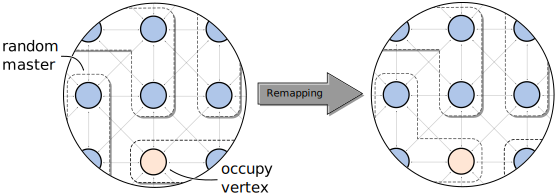
\includegraphics[width=\textwidth]{graphics/40_gol_remapping}
    \caption{Remapping of vertices to peers. A random master peer is
      determined by a consensus random number generation. The master
      dictates the vertex which will be occupied. Vertices of the
      graph are reannounced.}
    \label{fig:gol_remapping}
  \end{figure}



Even though, this the occupation scenario is an simple example it
shows remapping of vertices at runtime and therefore the power
to establish load balancing and fault tolerance techniques on
top of the system.

\cleardoublepage

%%% Local Variables:
%%% TeX-master: "diplom"
%%% End:
